% !TEX root = ../../main.tex

\chapter{Evaluation}
\label{chapter:evaluation-discussion}
This chapter shows Contribution \textbf{C.2}: A robust cost estimator for Amalur's factorized ML framework, and a comparison with the state-of-the-art in \autoref{sec:eval-model-evaluation}. Before that, we show how results were collected in \autoref{sec:experiment-setup}. The \hyperref[sec:eval-discussion]{third section} of this chapter provides an in-depth interpretation of the results as well as a critical view on the implications and limitations of this work.

\section{Experiment Setup}
\label{sec:experiment-setup}

\todo{Intro experimental environment, also serves as a guide on how to replicate the results}
This section goes into detail about anything needed to replicate the results. This includes the experimental environment (\hyperref[subsec:6-software]{Software}, \hyperref[subsec:6-datasets]{Datasets} \& \hyperref[subsec:6-hardware]{Hardware}),  and how the data was treated to ensure sound results for the cost estimators (\hyperref[subsec:6-validation-strategy]{validation strategy}). For more info and code please refer to the GitHub repository\footnote{\todo{TODO}}.

\subsection{Software}
\label{subsec:6-software}
The factorized ML framework (Amalur \cite{amalur}) is implemented in Python (3.10.4) and uses SciPy (1.8.0), NumPy (1.22.4) and CuPy (12.1.1). All experiments where ran in a Docker container with an image based on Nvidia's base image with CUDA 12.1.1 and Ubuntu 20.04\footnote{\href{https://hub.docker.com/layers/nvidia/cuda/12.1.1-devel-ubuntu20.04/images/sha256-5bd13c67a4479a1c13238b470d89a92937ce68ba5f21b930d50c463e3314f657?context=explore}{nvidia/cuda:12.1.1-devel-ubuntu20.04}}.

The choice to use CuPy as the backend for the factorized ML framework was made to ensure that the experiments could be run on both CPU and GPU. CuPy is a GPU-accelerated library for numerical computations that is compatible with NumPy and SciPy \cite{cupy_learningsys2017}. This allows for minimal changes to the codebase whether you are using GPU or CPU. To allow for exploitation of multiple cores for sparse matrix multiplication\footnote{\url{https://github.com/flatironinstitute/sparse_dot}} we use MKL (Intel Math Kernel Library) \cite{intel-mkl} as NumPy's backend for the CPU experiments.

For collecting the GPU metrics we use NVIDIA's Nsight Compute (ncu)\footnote{\url{https://docs.nvidia.com/nsight-compute/NsightComputeCli/index.html}} which is a command-line profiler that collects detailed performance metrics from the GPU. The metrics are collected in a CSV file for downstream analysis, detailed in \autoref{sec:5-feature-engineering}.

\subsection{Datasets}
\label{subsec:6-datasets}
The datasets used in the experiments are a mix of synthetic and real-world datasets. The synthetic datasets are used to generate a training set to train the cost estimators on. The real-world datasets are used to validate the cost estimators on unseen data.

\subsubsection{Synthetic Datasets}
To create the synthetic datasets with a wide variety of data characteristics the data generator from \cite{schijndel_cost_estimation} was used, which in turn is an adaptation of the data generator\footnote{\url{https://github.com/delftdata/valentine-data-fabricator}} from \cite{valentine-data-generator}.

In total, we generated $2415$ datasets, each being a two-table join. All other parameters were varied, the values are shown in \autoref{tab:6-synthetic-dataset-characteristics}.

\todo{Explain star schema (and show example)?}

\begin{table}[ht]
  \centering
  \begin{tabular}{llr}
    \toprule
    Data Characteristic             & Symbol    & Range                              \\ \midrule \midrule
    Target Sparsity                 & $e_T$     & $[ 0.0\text{,\ \ } 0.9]$           \\
    $S_1$ (Entity) table rows       & $r_{S_1}$ & $[ 40,000\text{,\ \ } 1,000,000]$  \\
    $S_1$ (Attribute) table rows    & $r_{S_2}$ & $[ 526\text{,\ \ } 1,000,000]$     \\
    $S_1$ (Entity) table columns    & $c_{S_1}$ & $[ 1\text{,\ \ } 50]$              \\
    $S_1$ (Attribute) table columns & $c_{S_2}$ & $[ 2\text{,\ \ } 50]$              \\
    Target table rows               & $r_T$     & $[ 60,000 \text{,\ \ } 1,000,000]$ \\
    Target table columns            & $c_T$     & $[ 11\text{,\ \ } 100]$            \\
    Tuple ratio                     & $\rho$    & $[ 1\text{,\ \ } 190]$             \\
    Feature ratio                   & $\tau$    & $[ 0.2\text{,\ \ } 1]$             \\
    Join Type                       & $j_T$     & Inner, left or outer.              \\
    Selectivity                     & $\sigma$  & $[ 1.0\text{,\ \ } 2.0]$           \\
    \bottomrule
  \end{tabular}
  \caption{Ranges of data characteristics for the generated synthetic datasets.}
  \label{tab:6-synthetic-dataset-characteristics}
\end{table}


\subsubsection{Real-world Datasets}
The synthetic datasets are convenient for testing and training purposes. However, to assess whether the cost estimators are generalizable to real-world data, we use real-world datasets for validation.

\paragraph{Project Hamlet \cite{2016-hamlet-sigmod}}
The Hamlet datasets are widely used in related literature \cite{2016-hamlet-sigmod, amalur, morpheus,orion_learning_gen_lin_models}. The Hamlet datasets are a set 7 datasets specifically designed to mimic data integration scenarios is an ML workflow. The original datasets where created to evaluate inner join scenario's. As we are also interested in other join types, some rows were removed from different source tables for these join types. The data characteristics of these datasets are shown in \autoref{tab:6-hamlet-characteristics}.

\todo{Right align numbers in table}
\begin{table}[ht]
  \centering
  \begin{tabular}{p{0.12\linewidth}rrrrrrr}
    \toprule
    Dataset$\rightarrow$ Characteristic $\downarrow$ & Book   & Expedia & Flight & Lastfm & Movie   & Walmart & Yelp   \\
    \midrule \midrule
    $r_T$                                            & 253120 & 942142  & 66548  & 343747 & 1000209 & 421570  & 215879 \\
    $c_T$                                            & 81663  & 52282   & 13669  & 55252  & 13348   & 2441    & 55606  \\
    $n$                                              & 2      & 3       & 4      & 2      & 2       & 3       & 2      \\
    $r_{S_1}$                                        & 27876  & 942142  & 66548  & 4999   & 6040    & 421570  & 11535  \\
    $r_{S_2}$                                        & 49972  & 11939   & 540    & 50000  & 3706    & 2340    & 43873  \\
    $r_{S_3}$                                        &        & 37021   & 3167   &        &         & 45      &        \\
    $r_{S_4}$                                        &        &         & 3170   &        &         &         &        \\
    $c_{S_1}$                                        & 28022  & 27      & 20     & 5019   & 9509    & 1       & 11706  \\
    $c_{S_2}$                                        & 53641  & 12013   & 718    & 50233  & 3839    & 2387    & 43900  \\
    $c_{S_3}$                                        &        & 40242   & 6464   &        &         & 53      &        \\
    $c_{S_4}$                                        &        &         & 6467   &        &         &         &        \\
    \bottomrule
  \end{tabular}
  \caption{}
  \label{tab:6-hamlet-characteristics}
\end{table}


\paragraph{TPCx-AI \cite{tpcx-ai}} We also evaluate on a scenario even more realistic than Hamlet, as it is based on a real-world benchmark used to evaluate end-to-end ML platforms. As that is not the focus of this work, we use only two out of the ten use cases, namely the first and the tenth use case. This benchmark also provides a data generator with scalable generation capabilities, through setting different \emph{Scale Factors} from \todo{lowest scale factor to the highest scale factor} we generated\todo{ How many datasets}. The data characteristics of the resulting datasets can be found in \autoref{tab:6-tpcx-ai-characteristics}.
\begin{table}[ht]
  \centering
  \begin{tabular}{lrr}
    \toprule
    {}                  & $r_T$ usecase1 & $r_S$ usecase1 \\
    dataset             &                &                \\
    \midrule
    scale\_factor\_0.01 & 3912340        & 519999         \\
                        &                & 3265601        \\
                        &                & 189263         \\
    scale\_factor\_0.5  & 23548828       & 3676955        \\
                        &                & 23036913       \\
                        &                & 1335985        \\
    scale\_factor\_1.0  & 33077704       & 5200000        \\
                        &                & 32577459       \\
                        &                & 1892589        \\
    scale\_factor\_3.0  & 56904679       & 9006664        \\
                        &                & 56419753       \\
                        &                & 3271336        \\
    \bottomrule
  \end{tabular}
  \caption{\todo{Finalize and add usecase2}}
  \label{tab:6-tpcx-ai-characteristics}
\end{table}

\todo{Explain use cases.}



\subsection{Hardware}
\label{subsec:6-hardware}
\todo{Table showing different machines tested on}

\begin{table}[ht]
  \centering
  \begin{tabular}{llllp{0.19\linewidth}}
    \toprule
    Experiment & Machine        & Compute Unit & Architecture & Experiment type \\
    \midrule
    \midrule
    GPU-P-1    & WIS ST4        & GPU A40      & Ampere       & profile         \\
    GPU-P-2    & AWS P3.2xlarge & GPU V100     & Volta        & profile         \\
    GPU-P-3    & Own desktop    & GPU 1660Ti   & Turing       & profile         \\
    GPU-T-1    & DAIC           & GPU A40      & Ampere       & runtime         \\
    GPU-T-2    & DAIC           & GPU V100     & Volta        & runtime         \\
    GPU-T-3    & DAIC           & GPU P100     & Pascal       & runtime         \\
    GPU-T-4    & DAIC           & GPU 2080Ti   & Turing       & runtime         \\
    GPU-T-5    & DAIC           & GPU 1080Ti   & Pascal       & runtime         \\
    CPU-T-1    & WIS ST4        & CPU 8 cores  & —            & runtime         \\
    CPU-T-2    & WIS ST4        & CPU 16 cores & —            & runtime         \\
    CPU-T-3    & WIS ST4        & CPU 32 cores & —            & runtime         \\
    \bottomrule
  \end{tabular}
  \caption{Overview of machines experiments will be run on.}
  \label{tab:my_label}
\end{table}

\subsection{Experiment Setting}
\todo{Number of iterations etc. (30 for experiments, e for profiling as it's included in ncu)}

\subsection{Validation Strategy}
\label{subsec:6-validation-strategy}
\todo{Explain how the collected metrics are divided into separate train \& test set to test generalizability}

\begin{figure}[ht]
  \centering
  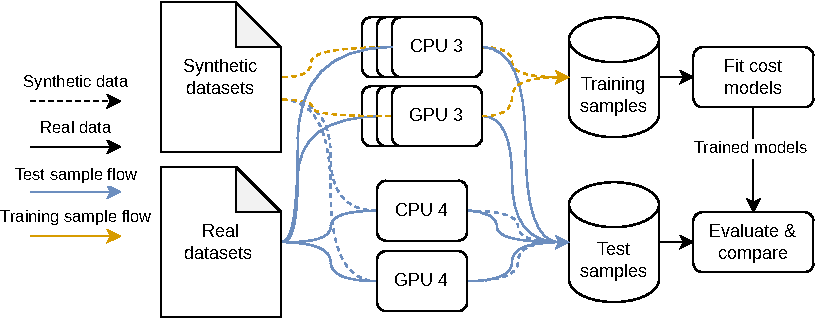
\includegraphics[width=0.8\linewidth]{chapters/06_evaluation/figures/experiment-pipeline.pdf}
  \caption{\todo{update} Overview of the planned experiments: combinations of datasets and machines we run the experiments
    on. }
  \label{fig:enter-label}
\end{figure}



\section{Cost Model Performance and Comparative Analysis}
\label{sec:eval-model-evaluation}

In this section we answer
\begin{itemize}
  \item[RQ.2] How can we accurately predict the optimal choice between factorized or materialized training of a Machine Learning model, on CPU and GPU, through leveraging knowledge about model, data, and hardware characteristics?
\end{itemize}

\subsection{Exploring Generalizability}
\subsubsection{Performance with New Datasets}

\subsubsection{Ablation Study}


\subsection{Cost Estimator Comparison}


\section{Discussion}
\label{sec:eval-discussion}

